\section{Coxalgie}

Alla base di un dolore all'anca possono esserci molteplici cause patologiche, di cui la più comune è l'\textbf{artros}i dell'anca. Ma spesso si ha la tendenza di sottovalutare tutte le altre cause di coxalgia e magari si fa erroneamente diagnosi di Coxartrosi perché non si sa da cos'altro possa derivare il dolore.

Per evitare questi errori ovviamente non si può prescindere dal fare una buona \emph{anamnesi} ed un buon \emph{esame obiettivo}. Solo in un secondo momento, saranno importanti le tecniche di imaging che devono infatti essere indirizzate dalle informazioni raccolte durante l'anamnesi e l'esame obiettivo.
\\\\
{[}Caso clinico 1: si consideri un paziente giovane (15-20 anni) che non ha altre patologie e che arriva all'attenzione del medico perché tutte le notti non riesce a dormire a causa di un dolore all'anca. In questo caso, nonostante le esigue informazioni, possiamo già essere indirizzati verso una neoplasia benigna: l'\textbf{osteoma osteoide}. Quest'ultima infatti si caratterizza proprio per questo dolore tipicamente notturno, è una neoplasia che non dà alcun tipo di metastasi ed è molto fastidiosa perché, finché non viene rimosso il tessuto tumorale, provoca un forte dolore gravativo ed urente nella sede di localizzazione.

Per confermare la diagnosi in questo caso si utilizza un criterio ex adiuvantibus: la somministrazione di \emph{aspirina}. Il dolore dovuto a questo tumore infatti recede dopo somministrazione di acido acetilsalicilico ma non dopo somministrazione di altri FANS.

Se il criterio ex adiuvantibus conferma la nostra diagnosi, (e cioè se il dolore recede dopo somministrazione di aspirina) andremo ad usare una TC per valutare dimensioni e localizzazione precisa della neoplasia benigna.{]}
\\\\
{[}Caso clinico 2: paziente di sesso maschile di 35-40 anni che riferisce un dolore sacro-iliaco. Riferisce inoltre di avere la psoriasi. Anche in questo caso è un dolore che si accentua di notte per poi affievolirsi durante il giorno. In questo caso però saremo orientati verso \textbf{un'artrite psoriasica sieronegativa}.{]}
\\\\
{[}Caso clinico 3: paziente di 12 anni abbastanza corpulento con dolore all'anca. Molto difficile che abbia un'artrite sieronegativa. Piuttosto, è più facile che abbia una \textbf{epifisiolisi}, una patologia dovuta a un difetto delle cartilagini di coniugazione, a causa del quale la testa del femore tende a scivolare verso il basso provocando dolore.{]}
\\\\
Da tutti questi casi clinici si capisce che l'anamnesi è assolutamente fondamentale per fare una buona diagnosi.

Uguale importanza riveste l'esame obiettivo. Con quest'ultimo si valutano le condizioni generali del paziente e, più in particolare, è possibile valutare:

\begin{itemize}
\item
  un eventuale disturbo della deambulazione.
\item
  l'ampiezza di movimento dell'anca, che se ridotta può orientare verso la diagnosi di coxartrosi.
\end{itemize}

Le \textbf{zoppie} sono di tre tipi:

\begin{itemize}
\item
  Zoppie \emph{di fuga}: il paziente "scappa" dall'appoggio in cui sente dolore e quindi fa il passo velocemente;
\item
  Zoppie \emph{da dismetria}: una gamba è più corta dell'altra (ad esempio a causa di una precedente frattura);
\item
  Zoppie \emph{da insufficienze glutee}: il gluteo non riesce a stabilizzare il bacino quando si fa un passo, per cui si ha la cosiddetta andatura anserina, "a papera", con il bacino che cade dall'altro lato quando si fa un passo.
\end{itemize}

Ci sono anche altre cause di zoppie, ma queste tre sono le più comuni.

{[}Caso clinico: paziente di sesso femminile, che pratica ginnastica artistica, ha dolore all'anca trocanterica. Durante la deambulazione si sente il classico "toc, cloc" dovuto al fatto che l'anca scatta avanti ed indietro. Siamo in questo caso nell'ambito delle anche a scatto trocanteriche o delle tendinoborsiti glutee.{]}

\subsection{Possibili cause di coxalgia}

Spesso, soprattutto in ambito fisiatrico, viene abusata la diagnosi di \textbf{sindrome del piriforme}. Quest'ultima è una patologia in cui il piriforme presenta un'\emph{ipertrofia} (primitiva o per cause secondarie, come ad esempio il piriforme di un atleta) e va a
\emph{comprimere il nervo sciatico} che passa tra il piriforme stesso ed il gemello superiore.

Questo causa un dolore che parte dalla zona sacro-iliaca e si irradia posteriormente nella gamba fino al ginocchio, più raramente fino al piede.

E' una patologia che ovviamente esiste, ma non è così comune. Per cui non bisogna abusarne in sede di diagnosi.

Esiste anche una patologia legata al legamento rotondo. Quest'ultimo ha una funzione trofica e stabilizzatrice sulla testa del femore in età infantile (queste funzioni vengono perse nel corso della vita). Quando questo legamento si lacera, si può sviluppare una sensazione dolorosa all'anca. E' quindi una \textbf{coxalgia da legamento rotondo}.

Nella \textbf{coxa vara} l'angolo formato dagli assi della testa e del corpo del femore è troppo piccolo, quasi un angolo retto. In questi soggetti le forze di flessione che si scaricano sulla testa del femore sono molto elevate e quindi aumenta enormemente il rischio di frattura della testa del femore.

La TC è un esame molto utile, ma a volte può risultare superfluo perché in alcuni casi la diagnosi è già ben evidente alla radiografia.

Questo esame va infatti utilizzato solo quando si hanno forti dubbi sul referto di una radiografia (esempio: sospetto di presenza di metastasi ossea).

\subsection{Tumore di Ewing}

\begin{figure}[!ht]
\centering
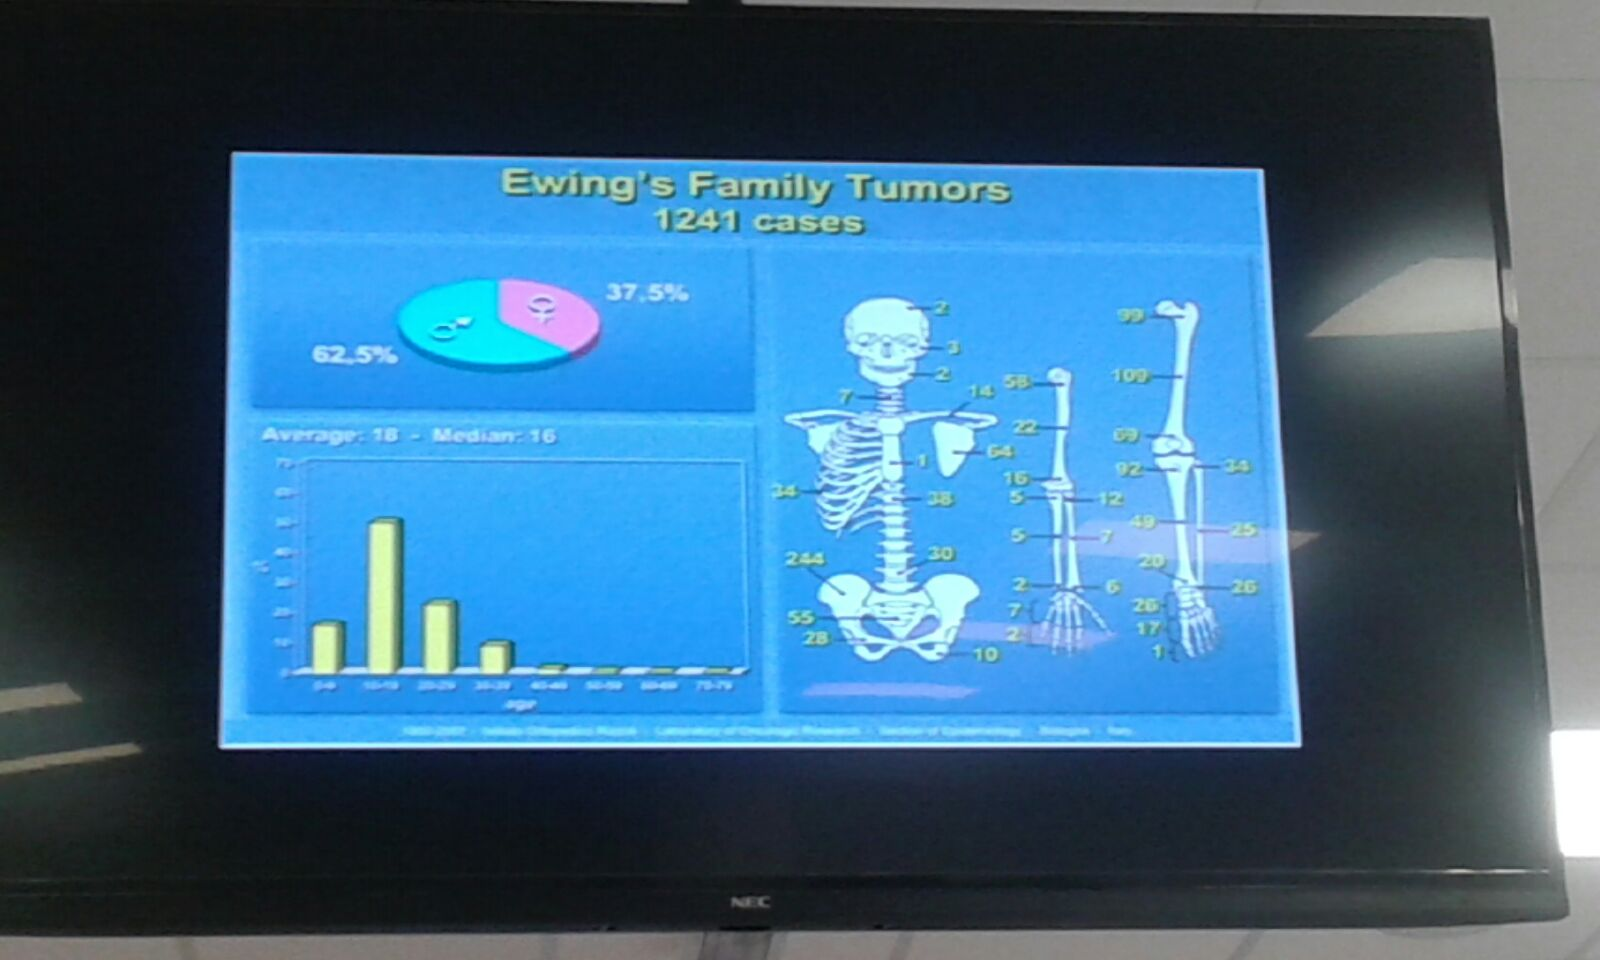
\includegraphics[width=0.4\textwidth]{019/image1.jpeg}
\end{figure}

Il tumore di Ewing è una neoplasia molto maligna con picco di incidenza tra i 10-19 anni ed i 20-29 anni. La possibilità di diagnosi di questo tumore va tenuta sempre in elevata considerazione in soggetti giovani, proprio perché questo tumore è molto aggressivo e può portare a morte in pochissimo tempo.

\section{Coxartrosi}

La coxatrosi è la più comune causa di coxalgia. Distinguiamo:

\begin{itemize}
\item
  coxartrosi \emph{primitive}, in cui non ci sono patologie che possono essere considerate causa dell'insorgenza della coxartrosi;
\item
  coxartrosi \emph{secondarie}, in cui è presente una patologia che è responsabile dell'avvento della coxartrosi.
\end{itemize}

Tra le patologie che causano le coxartrosi secondarie si trovano:

\begin{itemize}
\item
  tutte le malattie infiammatorie dismetaboliche: artrite reumatoide, artrite psoriasica, spondiloartrite anchilopoietica, lupus eritematoso sistemico, etc. ;
\item
  malattie infiammatorie croniche intestinali: morbo di Crohn, retto-colite ulcerosa;
\item
  necrosi della testa del femore;
\item
  impingement femoro-acetabolare;
\item
  algoneurodistrofia di Sudeck.
\end{itemize}

Le ultime tre cause di artrosi secondaria meritano una maggiore attenzione.

\subsection{Necrosi della testa del femore}

E' una patologia che si verifica quando l'afflusso di sangue alla testa del femore è compromesso. Anche in questo caso abbiamo moltissime cause:

\begin{itemize}
\item
  idiopatiche;
\item
  frattura del collo del femore, in questo caso vengono tranciati i vasi arteriosi che si occupano della vascolarizzazione della testa del femore;
\item
  post-traumatica, dovuta a traumi (come ad esempio un intervento chirurgico all'anca);
\item
  etilica, dovuta all'eccessivo consumo di bevande alcoliche;
\item
  post-cortisonica;
\item
  altre cause più rare.
\end{itemize}

\subsection{Impingement Femoro-Acetabolare}

\begin{figure}[!ht]
\centering
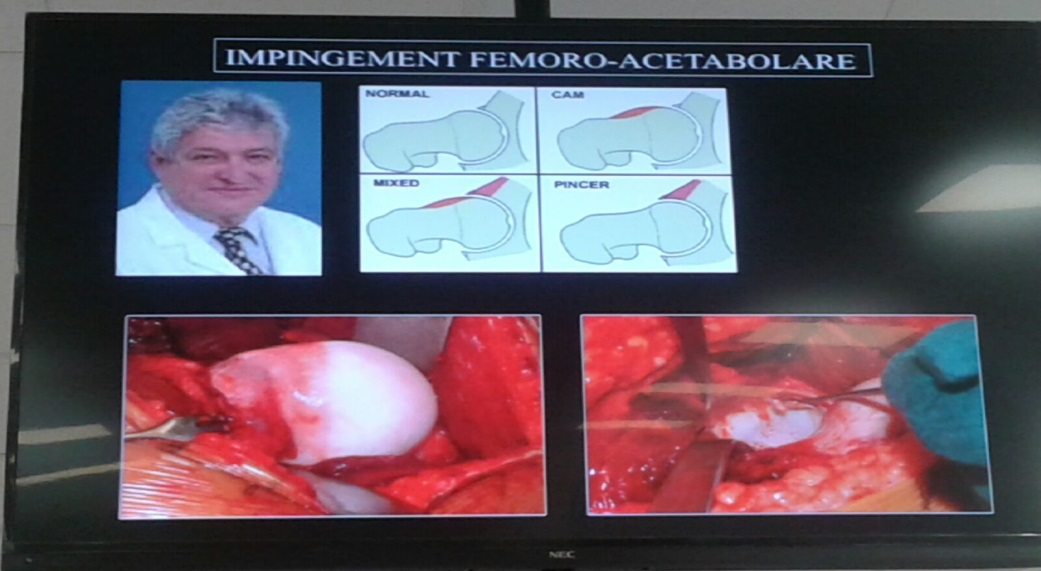
\includegraphics[width=0.4\textwidth]{019/image2.jpeg}
\end{figure}

L'impingement femoro-acetabolare è una patologia articolare che, nei soggetti affetti, aumenta enormemente il rischio di sviluppare artrosi in assenza di fattori di rischio (familiarità, obesità, lussazioni e sub-lussazioni dell'anca, fratture etc.).

Questo è dovuto al fatto che in questi soggetti sono presenti delle \textbf{anomalie di conformazione} della testa del femore o dell'acetabolo che non permettono un normale rapporto di adesione tra femore ed acetabolo.

Si conoscono tre tipi di impingement femoro-acetabolare:

\begin{itemize}
\item[1.]
  Impingement di \textbf{tipo Cam}: è presente una convessità ossea che sporge dalla testa del femore e, nei movimenti di flesso-estensione e di rotazione dall'anca, va a scontrarsi patologicamente con l'acetabolo e con la cartilagine articolare;
\item[2.]
  Impingement di \textbf{tipo Pincer}: è presente un acetabolo che avvolge troppo la testa del femore (normalmente dovrebbe coprire il 50\% della testa del femore) ed anche in questo caso ci sarà un continuo e patologico "scontro" tra testa del femore ed acetabolo;
\item[3.]
  Impingement di \textbf{tipo misto}: è la somma degli altri due impingement ed ovviamente in questo caso la patologia è ancora più grave.
\end{itemize}

\subsection{Algoneurodistrofia di Sudeck}

\begin{figure}[!ht]
\centering
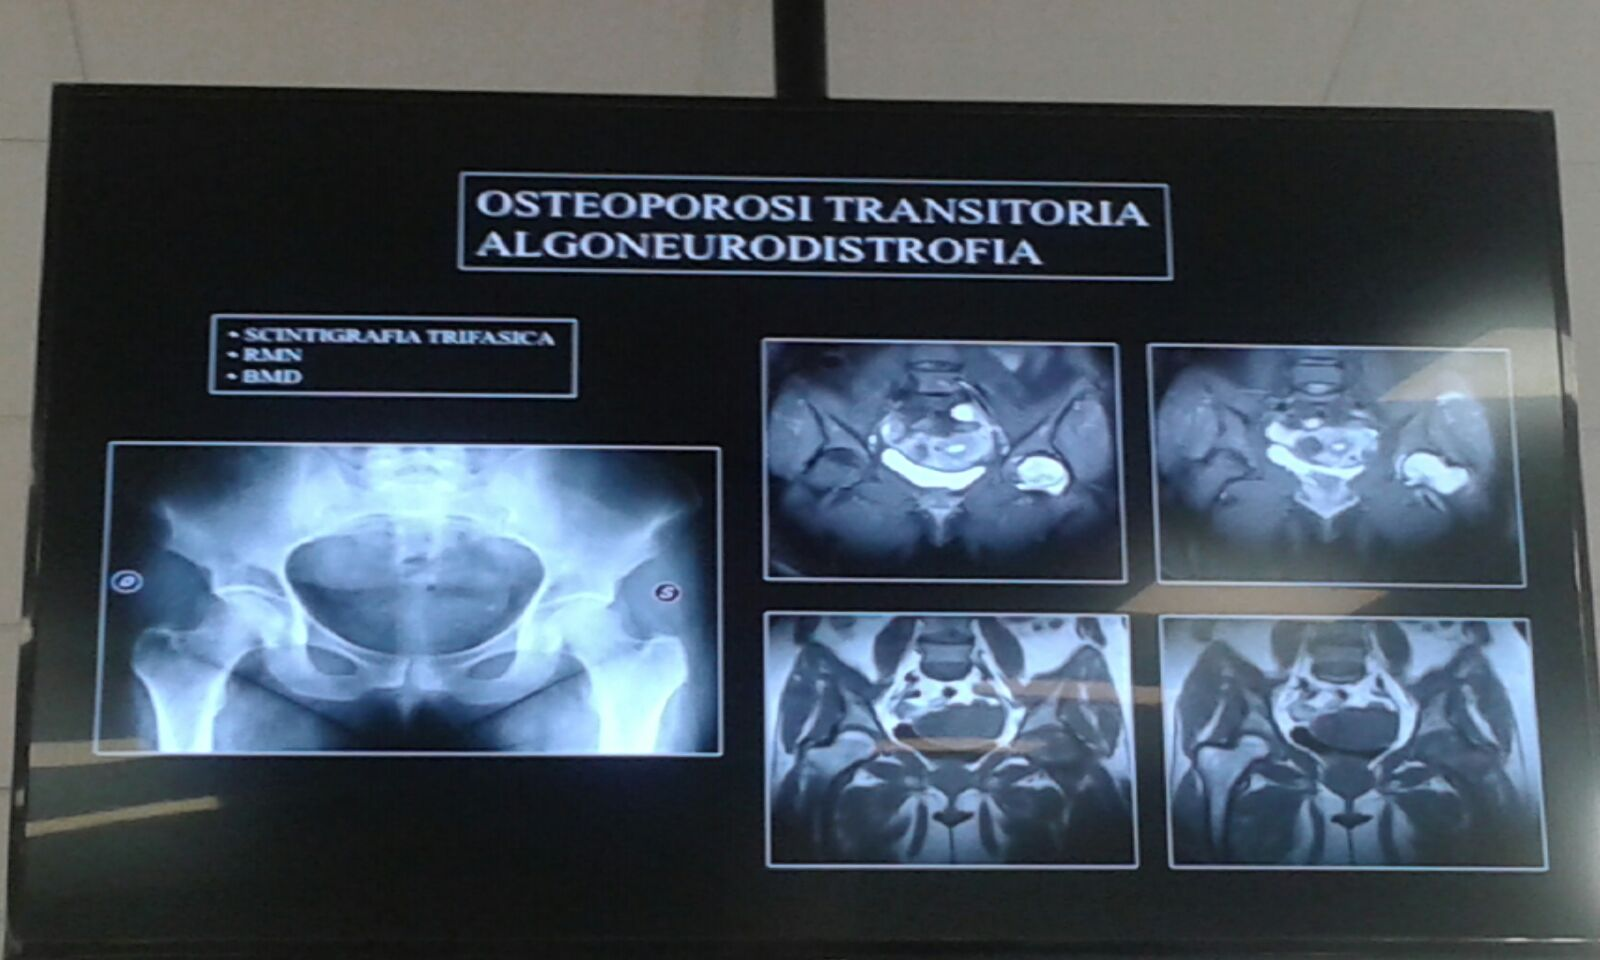
\includegraphics[width=0.4\textwidth]{019/image3.jpeg}
\end{figure}

E' un \textbf{cortocircuito} a livello \textbf{del sistema simpatico} che causa un circolo vizioso tra vasodilatazione e dolore.

Questo porta a rarefazione ossea fino a quando la demineralizzazione dell'osso è tale da configurare la cosiddetta \emph{atrofia vitrea}.

L'atrofia vitrea si può notare all'imaging: la zona della testa del femore è radiopaca (bianca), esattamente come lo è l'urina al centro dell'immagine. Questo perché c'è un voluminosissimo edema interstiziale nella zona interessata.

\subsection{Anatomia e Fisiologia dell'Anca}

L'anca è una struttura ossea che è data dall'incontro della
\textbf{testa del femore} con \textbf{l'acetabolo}. La ricettività di quest'ultimo nei confronti della testa del femore è aumentata dal \emph{cercine fibro-cartilagineo}. C'è poi \emph{sistema capsulare} che è un sistema di rinforzo dell'articolazione.

L'angolo di inclinazione tra l'asse della testa del femore e l'asse del corpo del femore è normalmente di 125\textsuperscript{o}. Inoltre esiste un angolo di declinazione di circa 25\textsuperscript{o} tra l'asse bicondilare e l'asse cervico-cefalico del femore.

Alterazioni di questi angoli possono riflettersi sulla biomeccanica dell'anca e provocare artrosi.

\begin{figure}[!ht]
\centering
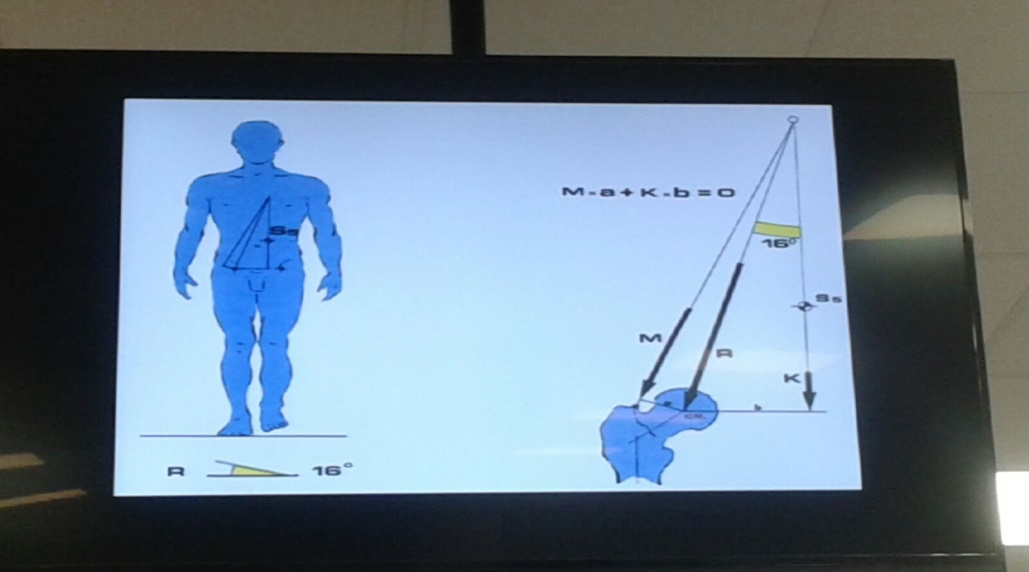
\includegraphics[width=0.4\textwidth]{019/image4.jpeg}
\end{figure}

L'immagine sopra mostra il cosiddetto \textbf{schema di Powell}, molto importante nell'impianto della protesi d'anca. Questo schema dice che, considerando una condizione di appoggio monopodalico, le forze che si scaricano sull'anca (vettore R nell'immagine) sono la sommatoria della forza di gravità (e quindi del peso corporeo, vettore K) e della forza generata dalla stabilizzazione del bacino da parte dei muscoli (vettore M).

La forza risultante R si scarica sulla testa del femore e, a seconda di come siano posizionate tra loro la testa del femore e l'acetabolo, R può variare e può quindi generare sollecitazioni verso l'una o l'altra parte della testa del femore.

\begin{itemize}
\item
  Ad esempio in una coxa valga (angolo di inclinazione tra testa del femore e corpo del femore maggiore di 125\textsuperscript{o}) ci sarà una patologica sollecitazione della parte superiore della testa del femore.
\item
  Al contrario una coxa vara (angolo di inclinazione minore di 125\textsuperscript{o}) solleciterà maggiormente la parte inferiore della testa del femore.
\end{itemize}

\begin{figure}[!ht]
\centering
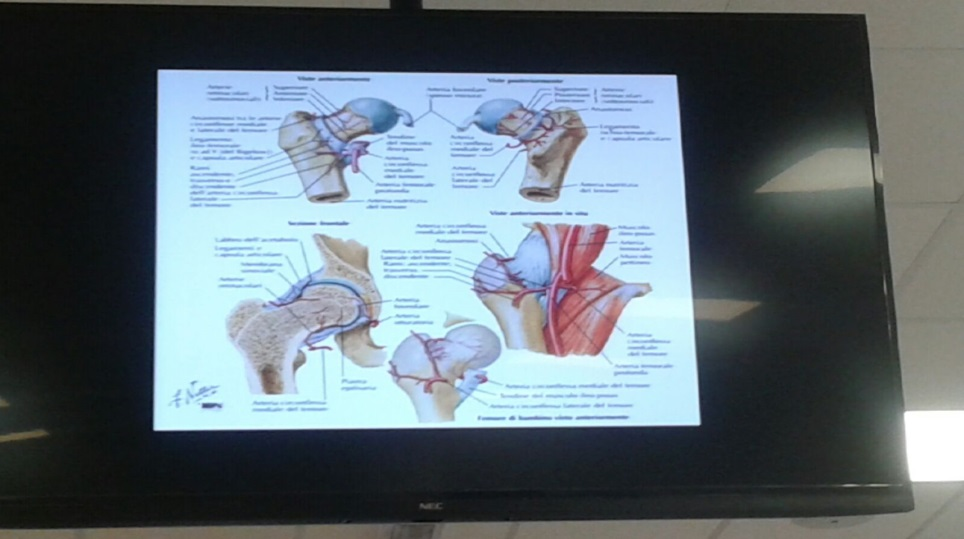
\includegraphics[width=0.4\textwidth]{019/image5.jpeg}
\end{figure}

Nell'immagine sopra si può vedere l'irrorazione della testa del femore, che è molto importante tenere a mente nei casi di osteonecrosi da frattura del collo del femore.

L'\textbf{irrorazione} prevede un \emph{anello alla base del collo} del femore da cui si diramano dei vasi che si fanno \emph{intracapsulari} decorrendo dal collo alla testa (che sono proprio quelli che vengono lesionati in caso in frattura del collo del femore).

\begin{figure}[!ht]
\centering
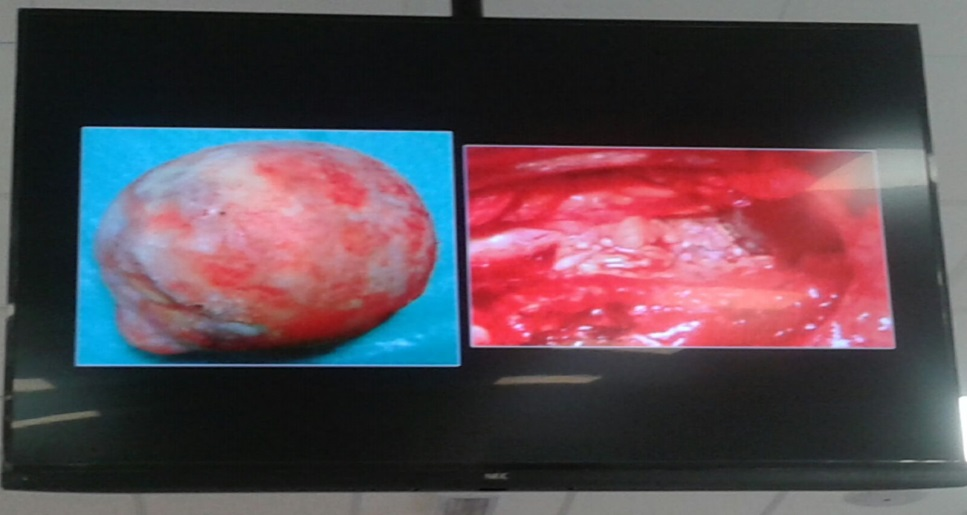
\includegraphics[width=0.4\textwidth]{019/image6.jpeg}
\end{figure}

\subsection{Fisiopatologia della Coxartrosi}

Nell'immagine vediamo una testa del femore. In condizioni fisiologiche dovremmo trovarla ricoperta di cartilagine, lucida e lucente.
Nell'immagine invece si vede bene la totale assenza di cartilagine.

L'\textbf{artrosi} è una patologia degenerativa.

E' diversa dall'\emph{artrite}, ma ci possono essere dei casi in cui le due patologie \emph{si sovrappongono}. In questo caso le artrosi hanno un aspetto di tipo "sinoviale".

Gli esami per confermare la diagnosi di artrite reumatoide saranno probabilmente negativi, però se andiamo ad incidere la capsula vediamo fuoriuscire del liquido che è dovuto ad una sinovite villosa.

\begin{itemize}
\item
  Nelle \textbf{coxartrosi primitive} non ci sono delle patologie scatenanti la coxartrosi stessa. In questo caso la testa del femore sarà uniformemente consumata ed ancora sferica, e dopo incisione non si trovano necrosi né liquido o altre caratteristiche che possono indirizzare verso una patologia che può avere scatenato l'artrosi.
\item
  Tra le \textbf{coxartrosi secondarie} più comuni si riconoscono:
\begin{itemize}
\item
  coxartrosi secondarie post-traumatiche (soprattutto da fratture);
\item
  coxartrosi secondarie a displasie congenite dell'anca (coxa vara e coxa valga);
\item
  coxartrosi secondarie ad impingement femoro-acetabolare;
\item
  coxartrosi secondarie ad artriti (infiammatorie, settiche etc..);
\item
  coxartrosi secondarie a malattie dell'infanzia come il morbo di Perthes e l'epifisiolisi.
\end{itemize}
\end{itemize}

Il \textbf{morbo di Perthes} è una patologia tipica dei bambini che si presentano con coxalgia verso i 6-7 anni. La causa della patologia risiede nel \emph{ridotto afflusso di sangue alla testa del femore}, la quale può andare incontro, prima, ad osteonecrosi e, successivamente, a frattura.

Questa sofferenza trofica porta all'appiattimento della testa del femore che può portare verso la coxartrosi.

L'\textbf{epifisiolisi} è anch'essa una patologia del bambino ma in questo caso è dovuta a un \emph{difetto delle cartilagini di coniugazione}, a causa del quale la testa del femore tende a scivolare verso il basso provocando dolore.

L'artrosi degenerativa dell'anca provoca una limitazione del movimento femorale. Ne consegue un importante impatto sulla funzione del cingolo pelvico e sul rachide lombare, poiché entrambi tentano di compensare la perdita di movimento a livello dell'anca.

\textbf{\emph{Valutazione}}

All'\textbf{ispezione} è evidente, soprattutto nelle forme più avanzate, un atteggiamento in adduzione, flessione e rotazione esterna, più raramente interna.

Alla \textbf{palpazione} possono riscontrarsi punti dolorosi dell'articolazione.

Alla \textbf{valutazione dei singoli movimenti} si ha una riduzione della flessione e, in misura maggiore e più precocemente, dell'abduzione, dell'intra ed extrarotazione e dell'estensione (il paziente fa fatica ad infilare le calze, a calzare le scarpe, a scendere o salire le scale). Negli stadi iniziali solo attività di maggior impegno articolare, come quelle sportive, determinano un aggravamento della situazione. Instaurata la malattia si avranno i \textbf{risultati a livello radiologico}: riduzione dell'interlinea articolare; gli osteofiti costituiscono un segno radiologico precoce e possono rilevarsi fenomeni di osteosclerosi e rarefazione a stampo (geodi).

L'\textbf{evoluzione} è lenta ed inesorabile e conduce ad un aggravamento progressivo con limitazione dei movimenti fino all'anchilosi. La degenerazione artrosica può avere molteplici cause, di particolare importanza è l'aspetto biomeccanico: una disfunzione dei sistemi articolare e neuromuscolare può dar luogo ad una cattiva distribuzione dei carichi, favorendo lo sviluppo di coxartrosi.

\subsection{Diagnosi di Coxartrosi}

E' basata innanzitutto sulla presenza di \textbf{dolore all'anca} (coxalgia) e sulla presenza di \textbf{zoppie}.

I sintomi sono il \textbf{dolore alla marcia}, avvertito all'inguine ed alla parte anteriore della coscia, il quale compare anche dopo essere rimasti seduti a lungo, mentre scompare in posizione orizzontale. Tipica è anche la \textbf{progressiva limitazione funzionale} prima dei
movimenti di \emph{intrarotazione} (difficoltà nell'uscire dalla vasca o nel salire su una bici), poi di quelli di \emph{abduzione} e quindi di \emph{adduzione}. Si accompagna ad una \emph{scoliosi lombare insorta
per compensazione} di una ``atteggiamento viziato'' in adduzione, flessione ed extrarotazione della coscia. L'Rx del bacino rivela un restringimento della rima articolare, con la direzione della dislocazione delle testa del femore indica inoltre se il danno cartilagineo è uniforme o meno. La diagnosi differenziale va posta con l'artrite dell'anca, in cui si ha un dolore di tipo flogistico, con aumento degli indici di flogosi ed erosioni, e le neoplasie dell'osso, in cui si ha un dolore simile ma che non recede a riposo.

Generalmente è abbastanza agevole la conferma diagnostica tramite la radiografia, ma in alcuni casi, se sono presenti dei dubbi, si può ricorrere alla RMN o alla TC.

Una ricostruzione tridimensionale può essere richiesta in preparazione ad un intervento chirurgico.

\subsection{Trattamento della Coxartrosi}

\subsubsection{Obiettivi}

\begin{itemize}
\item Riduzione del dolore e della reattività articolare
\item Aumento dell'ampiezza articolare
\item Miglioramento della stabilità articolare
\end{itemize}

\subsubsection{Principali strategie di intervento terapeutico}

\begin{itemize}
\item Tecniche articolari: trazione, traslazione, roll, swing, movimenti osteocinematici
\item Tecniche legamentose/tendinee: mobilizzazioni, trazioni
\item Tecniche muscolari: stretching, contrazioni isotoniche ed isometriche
\item Tecniche neuro dinamiche: sollevamento dell'arto inferiore esteso, propriocettiva
\item Combinazione di 2 o più tecniche
\item Massoterapia
\item Termoterapia, elettroterapia, ultrasuonoterapia, laserterapia, ortesi
\end{itemize}

\subsubsection{Riabilitazione prechirurgica dell'anca}

L'artroprotesi totale di anca prevede un percorso riabilitativo ben definito finalizzato a restituire la funzionalità dell'articolazione e possibilmente a migliorare quella precedente all'intervento.

Studi recenti hanno evidenziato come un trattamento pre-chirurgico dia le migliori garanzie post-intervento dal punto di vista della performance muscolare e motoria; ciò soprattutto in vista della ripresa dell'attività lavorativa e sociale del soggetto.

L'obiettivo del trattamento pre-chirurgico è far sì che il paziente si abitui sin da subito a svolgere esercizi per il recupero del tonotrofismo muscolare; in questo modo si presenterà all'intervento con una buona condizione muscolare e ciò accelererà i tempi di recupero.

Inoltre la riabilitazione pre-chirurgica educa il paziente all'utilizzo degli arti brachiali e alla gestione del carico.

Nella fase pre-operatoria il fisiatra deve
\begin{itemize}
\item valutare la sintomatologia dolorosa
\item valutare la capacità di deambulare con o senza ausili
\item valutare se dolore e impedimento possono causare disabilità e peggiorare gli atti della vita quotidiana. Esiste a questo scopo la Scala di valutazione WOMAC, che appunto valuta la sintomatologia dolorosa, l'arco di movimento dell'articolazione e la capacità del soggetto di attendere agli atti della vita quotidiana. Essa inoltre
permette di monitorare l'esito dell'intervento chirurgico e di quello riabilitativo.
\end{itemize}
Riassumendo, nella fase pre-operatoria il paziente va istruito su:
esercizi preintervento, consigli sulle corrette posture da assumere nel periodo di ricovero, uso di ausili e calzature adeguate per il percorso riabilitativo previsto. Inoltre, in base alle condizioni cliniche preintervento del paziente si deciderà la sede del trattamento riabilitativo. Se il soggetto è giovane e compliante e necessita di un rapido recupero va diretto verso un percorso ambulatoriale; un altro soggetto anziano e con comorbilità va invece riabilitato nelle strutture apposite o a casa.

\subsubsection{Riabilitazione postchirurgica dell'anca}
Il trattamento post-intervento deve
\begin{itemize}
\item prevenire i danni secondari all'immobilità
\item agire sul dolore
\item recuperare il tonotrofismo muscolare
\item recuperare il corretto schema del passo, perché questi pazienti già in partenza ce l'hanno alterato.
\end{itemize}

Il soggetto presenta infatti un' ipotonotrofia muscolare importante, soprattutto riguardante i muscoli glutei e ischio-crurali, quadricipite, tensore della fascia lata, adduttori e abduttori di anca che stabilizzano l'articolazione.

Il programma riabilitativo è alquanto denso e preciso, si divide in:

\paragraph{FASE DI MASSIMA PROTEZIONE (4-7 GIORNI)}

In questa fase è necessario:
\begin{itemize}
\item prevenire la dislocazione o la sublussazione, le complicanze polmonari;
\item raggiungere l'indipendenza nei trasferimenti prima della dimissione;
\item mantenere la forza degli arti superiori e dell'arto inferiore sano con esercizi attivi;
\item mantenere la mobilità dell'arto operato con esercizi di mobilizzazione passiva, in flessione, abduzione, rotazioni non controindicate dal tipo di accesso chirurgico;
\item prevenire una contrattura in flessione ponendo l'arto sano in massima flessione e lasciando rilassato l'arto operato, allungando i flessori dell'anca.
\end{itemize}

\subparagraph{1\textsuperscript{o} giorno postintervento}

Posizionare il paziente seduto sul letto, e consigliare di eseguire movimenti di flesso-estensione attiva degli adduttori e abduttori dell'arto controlaterale, in modo da stimolare nei giorni successivi gli stessi esercizi sull'arto operato. Secondo la scuola americana, il paziente va messo in carico dopo 24 h dall'intervento, questo grazie agli effetti della terapia antalgica infusiva; in Italia si è più cauti, ed il paziente viene verticalizzato in terza giornata. Questo perchè in primis vanno monitorate le complicanze vascolari dell'intervento: è vero che il paziente assume anticoagulanti e subisce un input-system
finalizzato alla ginnastica vascolare, ma gli imprevisti non vanno sottovalutati. Il paziente poi ha un catetere per il drenaggio dell'articolazione, e questo gli impedisce di deambulare (NB nelle protesi d'anca non si usa praticamente più,mentre si usa per quelle di ginocchio).

\subparagraph{2\textsuperscript{o} giorno}
\begin{itemize}
\item Il paziente si siede sul letto in posizione adeguata con le ginocchia leggermente flesse. Se il paziente è in buone condizioni si può sedere in poltrona, meglio se gestito con le gambe fuori dal letto. Infatti il
mantenimento del controllo del tronco aiuterà la successiva
verticalizzazione del paziente in terza giornata.
\item Rimozione dei drenaggi al fine di poter deambulare.
\end{itemize}

\subparagraph{3\textsuperscript{o} giorno}

Verticalizziamo il paziente e lo facciamo camminare con carico sfiorante o progressivo, usando un deambulatore con appoggio ascellare.

\subparagraph{4\textsuperscript{o} giorno}

Si prosegue il programma con deambulatore con appoggio ascellare.

\subparagraph{5\textsuperscript{o} giorno}

Se tutto funziona, il paziente usa due bastoni canadesi ad appoggio antibrachiale con un ritmo a 3 tempi. •

\subparagraph{6\textsuperscript{o} giorno}

Prosegue l'allenamento coi bastoni antibrachiali.

\subparagraph{7\textsuperscript{o} giorno}

Il paziente viene dimesso. Il periodo di ricovero è quindi di 6-8 giorni. Una volta dimessi, i pazienti possono essere inviati a domicilio o in una struttura pubblica o privata per il programma riabilitativo; qui svolgeranno un trattamento estensivo di 1 ora al giorno, oppure intensivo di 2 ore al giorno con personale dedicato (cosa non possibile in un reparto di ortopedia). Il setting riabilitativo dipende dalle condizioni del paziente e dalla compliance dei familiari, oltre che dall'assenza di barriere architettoniche a domicilio. A questo scopo il
servizio territoriale invia un terapista a domicilio che, in 5 sedute, istruirà il paziente e i familiari su come usare il deambulatore e i bastoni canadesi antibrachiali. Spesso infatti il paziente esce dall'ospedale usando ancora il deambulatore ad appoggio ascellare, e la figura del terapista a domicilio diventa quindi essenziale. Riassumendo, il trattamento post-intervento riabilita la muscolatura glutea, gli adduttori di coscia e il quadricipite. Per fare ciò si deve recuperare l'arco di movimento e istruire il paziente sull'uso dei bastoni canadesi, che non andrebbero abbandonati prima di 1mese-1 mese e mezzo.
E' utile poi fare il controllo della protesi dopo 30 giorni
dall'intervento e somministrare al paziente la scala di valutazione WOMAC per avere un numero che quantifichi il recupero. NB In caso di Problemi sul trasferimento del paziente nel centro riabilitativo (mancanza del posto), il trattamento deve proseguire nel reparto di ortopedia dove questi è stato operato.

\paragraph{FASE DI MODERATA E MINIMA PROTEZIONE (8 giorni/6-12 settimane)}

È necessario recuperare la forza, la resistenza ed il movimento articolare dell'arto operato con:
\begin{itemize}
\item Mobilizzazione passiva seguendo la corretta artrocinematica dell'anca
\item Flesso estensione di anca e ginocchio strisciando il tallone sul lettino
\item Flessione dell'anca a ginocchio esteso, assistita poi attiva, infine contro resistenza
\item Abduzione dell'anca sul piano del letto, poi con resistenza elastica, infine contro gravità in decubito laterale controlaterale all'arto operato
\item Esercizio del ponte, prima con entrambe le gambe, poi con l'arto operato flesso e l'altro esteso e sollevato dal lettino
\item Esercizi di flessione e abduzione attiva dell'arto operato in posizione eretta - qualora sia concesso il carico monopodalico, si possono eseguire mini-squat, passi laterali e affondi - migliorare l'equilibrio mediante esercizi su superfici instabili (tavole propriocettive), incrementare il carico durante la deambulazione e correggere eventuali compensi; - migliorare la resistenza
cardiorespiratoria con attività aerobiche, - preparare il paziente al ritorno alle normali attività con esercizi funzionali come salire e scendere le scale, percorrere a piedi distanze crescenti.
\item
  In presenza di una coxartrosi secondaria, ove possibile si cerca di eliminare la causa.
\end{itemize}

Ad esempio se il paziente ha un impingement femoro-acetabolare si può cercare di ridurlo con un intervento di artroscopia.

\begin{itemize}
\item
  Negli altri casi l'alternativa è l'\textbf{osteotomia} eseguita sull'acetabolo, sulla testa del femore o su entrambi.
\item
  Quando però l'artrosi è troppo avanzata, non si può fare a meno di fare un intervento che preveda l'impianto di una \textbf{protesi d'anca}. La protesi ha il compito di ripristinare la corretta geometria dell'anca per ripristinare la funzione e per ridurre l'usura che aveva causato la coxartrosi.
\end{itemize}

Normalmente nell'artrosi d'anca non si possono fare delle endoprotesi parziali, ma la protesi è sempre e comunque una \emph{protesi totale}.
Questa prevede la sostituzione della testa del femore e dell'acetabolo.

Le \emph{endoprotesi parziali} possono essere invece una valida possibilità in un paziente anziano che abbia subito una frattura del collo del femore. In quel caso si può sostituire soltanto il femore lasciando stare l'acetabolo.

Il 94\% delle protesi d'anca impiantate in Emilia Romagna sono ancora sopravviventi dopo 10 anni.

Nell'impianto di una protesi è di fondamentale importanza lo \textbf{schema di Powell}. Bisogna infatti usare una protesi che, una volta impiantata, generi un sistema il più possibile conforme allo schema di Powell. Se questo non succede ovviamente la protesi può non avere il successo terapeutico sperato.

Per questo motivo, non esiste una protesi che vada bene per qualsiasi
paziente. Esistono infatti moltissimi tipi di protesi con
caratteristiche diverse ed è di fondamentale importanza la scelta di una
protesi che sia adeguata per un determinato paziente.

Nella scelta della protesi vanno considerati parametri come

\begin{itemize}
\item
  l'età
\item
  il sesso
\item
  la morfologia ossea
\item
  la qualità ossea.
\end{itemize}

Inoltre, la ricostruzione tridimensionale dell'anca del paziente può essere di grande aiuto.

La \textbf{chirurgia mini-invasiva} è una tecnica con la quale si cerca di danneggiare al minimo i tessuti sani (in particolare il tessuto muscolare) per far sì che possano essere ben ricostruiti.

E' una metodica utile ma purtroppo non può essere utilizzata in tutti i casi.
